\documentclass[11pt,border=5pt]{standalone}
\usepackage{fontspec}
\setmainfont{cmunrm.otf}[BoldFont=cmunbx.otf,ItalicFont=cmunti.otf,BoldItalicFont=cmunbi.otf]
\usepackage{amsmath}
\usepackage{unicode-math}
\setmathfont{NewCMMath-Regular.otf}
\usepackage{tikz}
\usetikzlibrary{arrows.meta,patterns,angles,quotes}
\begin{document}
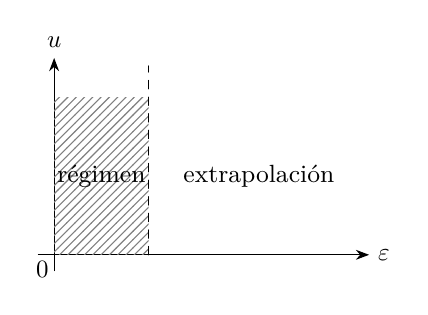
\begin{tikzpicture}[>=Stealth,font=\small,line cap=round,line join=round]
\draw[->,thin] (-0.2,0) -- (4,0) node[right] {$\varepsilon$};
\draw[->,thin] (0,-0.2) -- (0,2.5) node[above] {$u$};
\node at (-0.14,-0.18) {$0$};
\fill[pattern=north east lines,pattern color=gray] (0,0) rectangle (1.2,2);\draw[dashed] (1.2,0)--(1.2,2.4);\node at (0.6,1) {régimen};
\node at (2.6,1) {extrapolación};

\end{tikzpicture}
\end{document}
